\documentclass[11pt]{article}
\usepackage{euscript}
\usepackage{amsmath}
\usepackage{amsthm}
\usepackage{amssymb}
\usepackage{epsfig}
\usepackage{xspace}
\usepackage{amsmath,amssymb,amsthm}
\usepackage{graphicx}
\usepackage[margin=1in]{geometry}
\usepackage{fancyhdr}
\usepackage{color}
\usepackage{url}
\usepackage{bbm}
%%%%%%%%%%%%%%%%%%%%%%%%%%%%%%%%%
\setlength{\textheight}{9in}
\setlength{\topmargin}{-0.600in}
\setlength{\headheight}{0.2in}
\setlength{\headsep}{0.250in}
\setlength{\footskip}{0.5in}
\flushbottom
\setlength{\textwidth}{6.5in}
\setlength{\oddsidemargin}{0in}
\setlength{\evensidemargin}{0in}
\setlength{\columnsep}{2pc}
\setlength{\parindent}{1em}
\setlength{\parindent}{0pt}
\setlength{\parskip}{5pt plus 1pt}
\setlength{\headheight}{13.6pt}
%%%%%%%%%%%%%%%%%%%%%%%%%%%%%%%%%
\usepackage{epsfig}
\usepackage{xspace}
\usepackage{amsmath,amssymb,amsthm}
\usepackage{graphicx}
\usepackage[margin=1in]{geometry}
\usepackage{fancyhdr}
\usepackage{color}
\usepackage{url}
%%%%%%%  For drawing trees  %%%%%%%%%
\usepackage{tikz}
\usetikzlibrary{calc, shapes, backgrounds}
%%%%%%%%%%%%%%%%%%%%%%%%%%%%%%%%%
\setlength{\textheight}{9in}
\setlength{\topmargin}{-0.600in}
\setlength{\headheight}{0.2in}
\setlength{\headsep}{0.250in}
\setlength{\footskip}{0.5in}
\flushbottom
\setlength{\textwidth}{6.5in}
\setlength{\oddsidemargin}{0in}
\setlength{\evensidemargin}{0in}
\setlength{\columnsep}{2pc}
\setlength{\parindent}{1em}
\setlength{\parindent}{0pt}
\setlength{\parskip}{5pt plus 1pt}
\setlength{\headheight}{13.6pt}
%%%%%%%%%%%%%%%%%%%%%%%%%%%%%%%%%
\newcommand{\eps}{\varepsilon}
\renewcommand{\c}[1]{\ensuremath{\EuScript{#1}}}
\renewcommand{\b}[1]{\ensuremath{\mathbb{#1}}}
\renewcommand{\theenumi}{\alph{enumi}}
\newcommand{\s}[1]{\textsf{#1}}
\newcommand{\E}{\textbf{\textsf{E}}}
\renewcommand{\Pr}{\textbf{\textsf{Pr}}}
\newcommand\question[2]{\vspace{.25in}\hrule\textbf{#1: #2}\vspace{.5em}\hrule\vspace{.10in}}
\renewcommand\part[1]{\vspace{.10in}\textbf{(#1)}}
\newcommand\algorithm{\vspace{.10in}\textbf{Algorithm: }}
\newcommand\correctness{\vspace{.10in}\textbf{Correctness: }}
\newcommand\runtime{\vspace{.10in}\textbf{Running time: }}
\pagestyle{fancyplain}

\graphicspath{ {.} }

\lhead{\textbf{\NAME\ (\UNI)}}
\chead{\textbf{HW\HWNUM}}
\rhead{COMS W4721, \today}


\newcommand\NAME{Daniel Kronovet}  
\newcommand\UNI{003349897}    
\newcommand\HWNUM{02}          

\begin{document}

%%%%%%%%%%%%%%%%%%%%%%%%%%%%%%%%%%%%%%%%%%%%%%%%%%%%
%%%%%%%%%%%%%%%%%%%%%%%%%%%%%%%%%%%%%%%%%%%%%%%%%%%%
%%%%%%%%%%%%%%%%%%%%%%%%%%%%%%%%%%%%%%%%%%%%%%%%%%%%

\section*{Problem 1 (multiclass logistic regression)}

\begin{enumerate}
\item Write out the log likelihood $L$ of data $(x_1, y_1), . . . , (x_n, y_n)$ using an i.i.d. assumption.

\[
L = \prod_{i=1}^{n} \prod_{j=1}^{k} (\frac{e^{x_i^Tw_j}}{\sum_{l=1}^k e^{x_i^Tw_l}})^{\mathbbm{1}(y_i = j)}
\]

First, we observe that while $p(y|x, w_1, ..., w_n)$ is a product of the likelihood of each $w$, the indicator effectively cancels out every $w_i, i \neq c$ as $z^{\mathbbm{1}(y = c)} = z^0 = 1$, where $c$ is the true class of data point $x_i$. Furthermore, since we are only considering $x_i$ in the context of the correct class, we can eliminate the indicator function also.

With that in mind, we can cast the joint probability of the data as:

\[
L = \prod_{i=1}^{n} (\frac{e^{x_i^Tw_i}}{\sum_{j=1}^k e^{x_i^Tw_j}})
\]

Taking the natural log of this, we have:

\[
\mathcal{L} = lnL = \sum_{i=1}^{n} ln(\frac{e^{x_i^Tw_i}}{\sum_{j=1}^k e^{x_i^Tw_j}})
\]

\[
\mathcal{L} = \sum_{i=1}^{n} (x_i^Tw_i - ln({\sum_{j=1}^k e^{x_i^Tw_j}}))
\]

\item Calculate $\nabla_{w_i} \mathcal{L}$ and $\nabla^2_{w_i} \mathcal{L}$.

\section*{$\nabla_{w_i} \mathcal{L}$}

Beginning with the log likelihood:

\[
lnL = \sum_{i=1}^{n} (x_i^Tw_i - ln({\sum_{j=1}^k e^{x_i^Tw_j}}))
\]

\[
\nabla_{w_i}\mathcal{L} = \sum_{i=1}^{n} (x_i - \frac{1}{\sum_j^k e^{x_i^Tw_j}} (e^{x_i^Tw_i}) x_i)
\]

\[
\nabla_{w_i}\mathcal{L} = \sum_{i=1}^{n}(x_i) (1 - \frac{e^{x_i^Tw_i}}{\sum_j^k e^{x_i^Tw_j}})
\]

The numerator $e^{x_i^Tw_i}$ makes sense because we take the gradient with respect to $w_i$. Therefore, the terms of the summation are 0 for every $w_j, w_j \neq w_i$.
To interpret the gradient, we see how the greater the probability of $x_i$, the smaller $\nabla_{w_i}lnL$, or the less of an impact a change in $w_i$ will have on the likelihood.

\section*{$\nabla^2_{w_i} \mathcal{L}$}

To calculate the Hessian, we consider each term $\mathcal{L}_l$ separately, and calculate the second derivative for that term.

This gives us:

\[
\nabla_{w_i} \mathcal{L}_l = \sum_{i=1}^{n}(x_{il}) (1 - \frac{e^{x_i^Tw_i}}{\sum_j^k e^{x_i^Tw_j}})
\]

Using the quotient rule to take the derivative of the rightmost term:

\[
\nabla_{w_i}^2 \mathcal{L}_l = \sum_{i=1}^{n}(x_{il}) (1 - \frac{x_i e^{x_i^Tw_i}\sum_j^k e^{x_i^Tw_j} - x_i e^{2x_i^Tw_i}}{(\sum_j^k e^{x_i^Tw_j})^2})
\]

\[
\nabla_{w_i}^2 \mathcal{L}_l = \sum_{i=1}^{n}(x_{il}) (1 - \frac{x_i (e^{x_i^Tw_i}\sum_j^k e^{x_i^Tw_j} - e^{2x_i^Tw_i})}{(\sum_j^k e^{x_i^Tw_j})^2})
\]

If we set $c = e^{x_i^Tw_i}\sum_j^k e^{x_i^Tw_j} - e^{2x_i^Tw_i}$ and $d = (\sum_j^k e^{x_i^Tw_j})^2$, both scalars, we have:

\[
\nabla_{w_i}^2 \mathcal{L}_l = \sum_{i=1}^{n}(x_{il}) (1 - \frac{x_i c}{e})
\]

As $x_{il}$ is also a scalar (element $l$ of gradient vector $ \mathcal{L}$), and $x_i$ is a vector, this expression evaluates to a vector. Thus, evaluating this expression for every $\mathcal{L}_l$ in $(1, 2, ... d)$ where $d$ is the number of elements (dimensions) in  $\mathcal{L}$, (and summing across every $x_i$ in $X$), we generate the Hessian matrix:

\[
\nabla_{w_i}^2 \mathcal{L} = [\nabla_{w_i}^2 \mathcal{L}_1, \nabla_{w_i}^2 \mathcal{L}_2, ..., \nabla_{w_i}^2 \mathcal{L}_d]^T
\]

\end{enumerate}

\section*{Problem 2 (Gaussian kernels)}

To begin:

\[
K(u, v) = \int \phi_t(u) \phi_t(v) dt
\]

Expanding:

\[
K(u, v) = \int \frac{1}{(2\pi\beta^\prime)^{d/2}}e^{({- \frac{||u - t||^2}{2\beta^\prime}})} \frac{1}{(2\pi\beta^\prime)^{d/2}}e^{({- \frac{||v - t||^2}{2\beta^\prime}})} dt
\]

Rearranging:

\[
K(u, v) = \int \frac{1}{(2\pi\beta^\prime)^{d/2}}e^{({- \frac{||u - t||^2 + ||v - t||^2}{2\beta^\prime}})} dt
\]

Focusing only on the terms in the exponent:

\[
||u - t||^2 + ||v - t||^2
\]

\[
= u^Tu + t^Tt - 2u^Tt + v^Tv + t^Tt - 2v^Tt
\]

\[
= 2||t||^2 - 2(u + v)^Tt + ||u||^2 + ||v||^2
\]

\[
= ||t||^2 - (u + v)^Tt + \frac{||u||^2}{2} + \frac{||v||^2}{2}
\]

Then we complete the square:

\[
= ||t||^2 - (u + v)^Tt + ||\frac{u+v}{2}||^2 -  ||\frac{u+v}{2}||^2 + \frac{||u||^2}{2} + \frac{||v||^2}{2}
\]

\[
= ||t - \frac{u + v}{2}||^2 - ||\frac{u+v}{2}||^2 + \frac{||u||^2}{2} + \frac{||v||^2}{2}
\]

Placing this back into context:

\[
K(u, v) = \int \frac{1}{(2\pi\beta^\prime)^{d/2}}e^{-\frac{1}{2\beta^\prime}(||t - \frac{u + v}{2}||^2 - ||\frac{u+v}{2}||^2 + \frac{||u||^2}{2} + \frac{||v||^2}{2})} dt
\]

Rearranging, we can form a Gaussian in $t$:

\[
K(u, v) = \frac{1}{(2\pi\beta^\prime)^{d/2}}e^{-\frac{1}{2\beta^\prime}(- ||\frac{u+v}{2}||^2 + \frac{||u||^2}{2} + \frac{||v||^2}{2})} \int \frac{1}{(2\pi\beta^\prime)^{d/2}}e^{-\frac{1}{2\beta^\prime}(||t - \frac{u + v}{2}||^2)} dt
\]

The term to be integrated is now a well-formed Gaussian in $t$. We can integrate this to 1, leaving us with:

\[
K(u, v) = \frac{1}{(2\pi\beta^\prime)^{d/2}}e^{-\frac{1}{2\beta^\prime}(- ||\frac{u+v}{2}||^2 + \frac{||u||^2}{2} + \frac{||v||^2}{2})}
\]

Returning to the exponent, we have:

\[
- ||\frac{u+v}{2}||^2 + \frac{||u||^2}{2} + \frac{||v||^2}{2}
\]

\[
\frac{||u||^2}{2} - ||\frac{u+v}{2}||^2  + \frac{||v||^2}{2}
\]

\[
\frac{||u||^2}{2} - (\frac{u+v}{2})^T(\frac{u+v}{2})  + \frac{||v||^2}{2}
\]

\[
\frac{||u||^2}{2} - \frac{(u+v)^T(u+v)}{4} + \frac{||v||^2}{2}
\]

\[
\frac{||u||^2}{2} - \frac{||u||^2 + 2u^Tv + ||v||^2}{4}  + \frac{||v||^2}{2}
\]

\[
\frac{2||u||^2 - ||u||^2 - 2u^Tv - ||v||^2 + 2||v||^2}{4}
\]

\[
\frac{||u||^2 - 2u^Tv  + ||v||^2}{4}
\]

\[
\frac{||u - v||^2}{4}
\]

Returning to context:

\[
K(u, v) = \frac{1}{(2\pi\beta^\prime)^{d/2}}e^{-\frac{1}{2\beta^\prime}(\frac{||u - v||^2}{4})}
\]

\[
K(u, v) = \frac{1}{(2\pi\beta^\prime)^{d/2}}e^{-(\frac{||u - v||^2}{8\beta^\prime})}
\]

Now, we define $\alpha = f_1(\beta^\prime)$ and $\beta = f_2(\beta^\prime)$, to achieve our desired result:

\[
K(u, v) = \alpha e^{-(\frac{||u - v||^2}{\beta})}
\]

\section*{Problem 3 (Classification)}

\begin{table}[!th]
\centering
\begin{tabular}{|l|r|}
\hline
K &  Acc \\
\hline
1 & .948 \\
2 & .93  \\
3 & .918 \\
4 & .902 \\
5 & .894 \\
\hline
\end{tabular}
\caption{Prediction accuracy for KNN}
\label{ex:table}
\end{table}

\begin{table}[!th]
\centering
\begin{tabular}{|c|c|c|}
\hline
Class & Prediction & Image \\
\hline
3 & 8 & 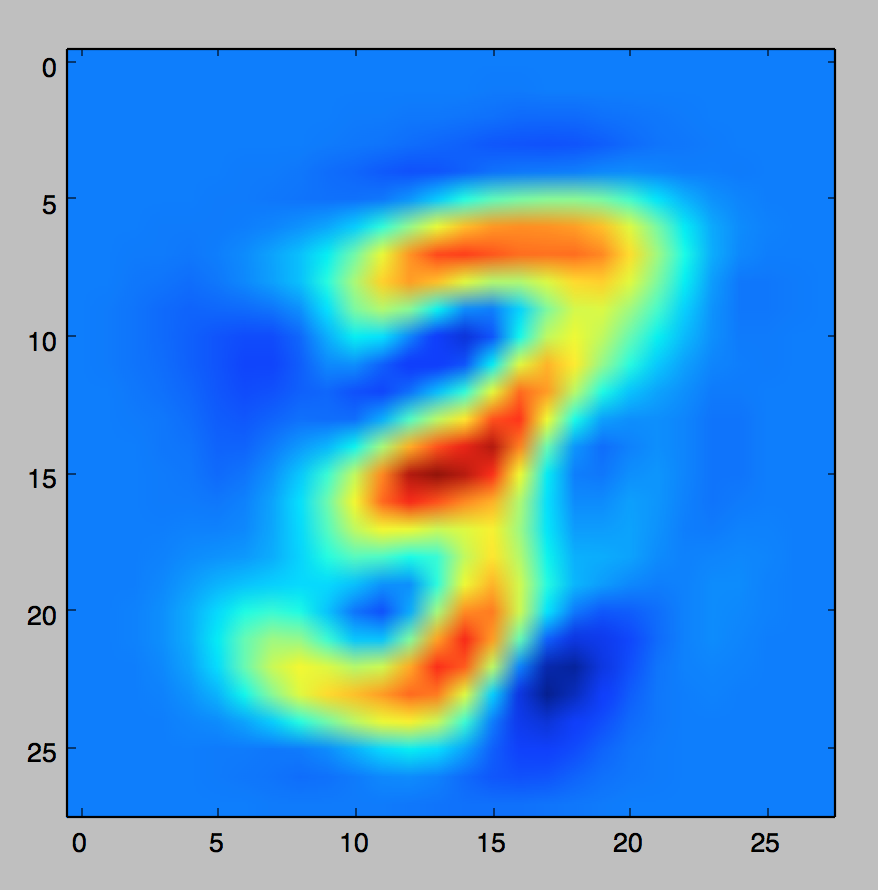
\includegraphics[scale=.15]{images/knn1_3_8.png} \\
\hline
5 & 4 & 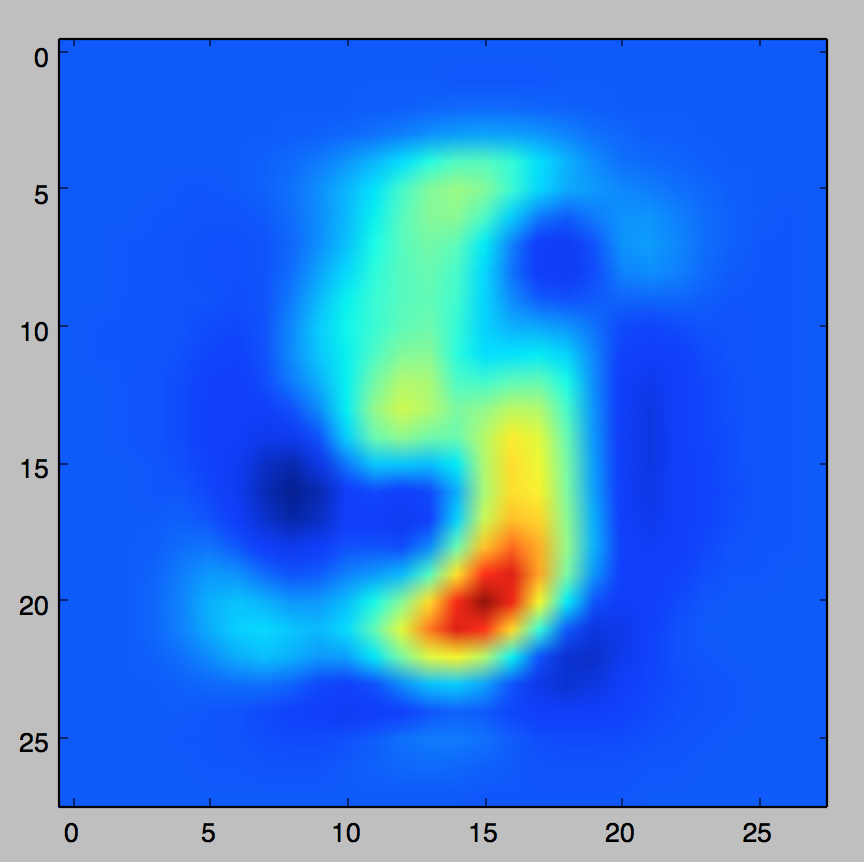
\includegraphics[scale=.15]{images/knn1_5_4.png} \\
\hline
8 & 9 & 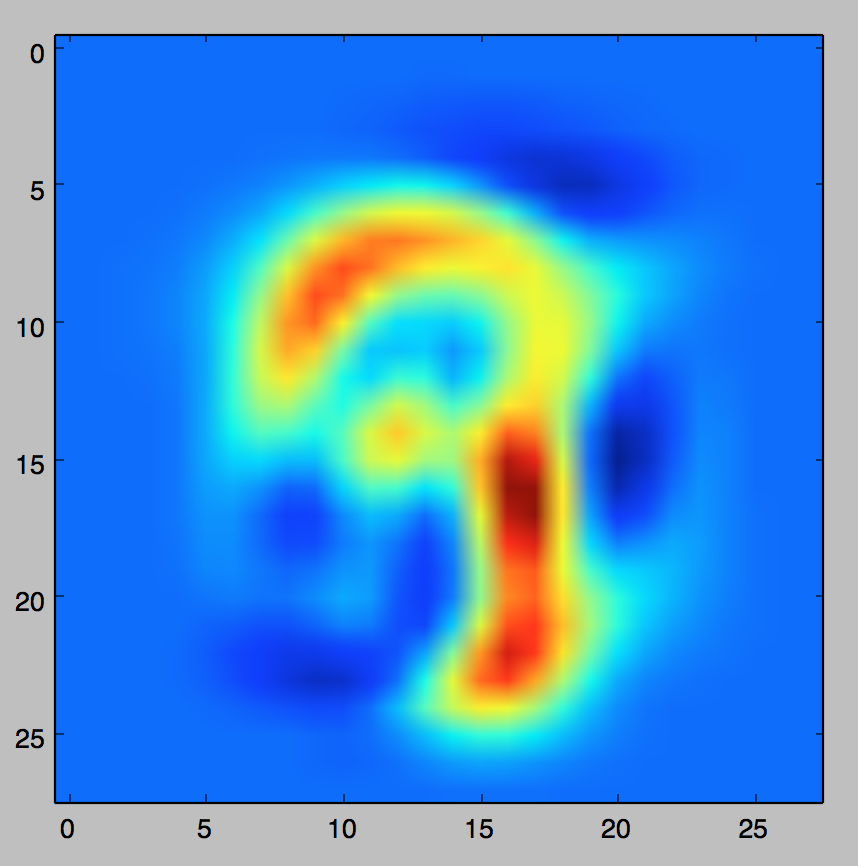
\includegraphics[scale=.15]{images/knn1_8_9.png} \\
\hline
\end{tabular}
\caption{Misclassified examples for K=1}
\label{ex:table}
\end{table}

\begin{table}[!th]
\centering
\begin{tabular}{|c|c|c|}
\hline
Class & Prediction & Image \\
\hline
3 & 7 & 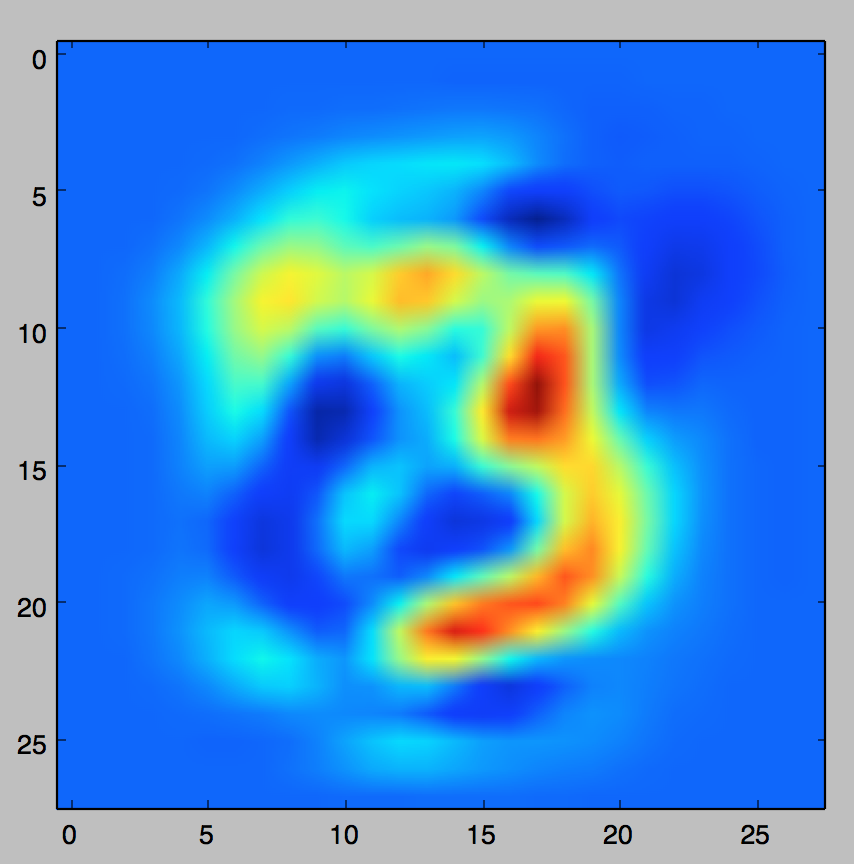
\includegraphics[scale=.15]{images/knn3_3_7.png} \\
\hline
8 & 3 & 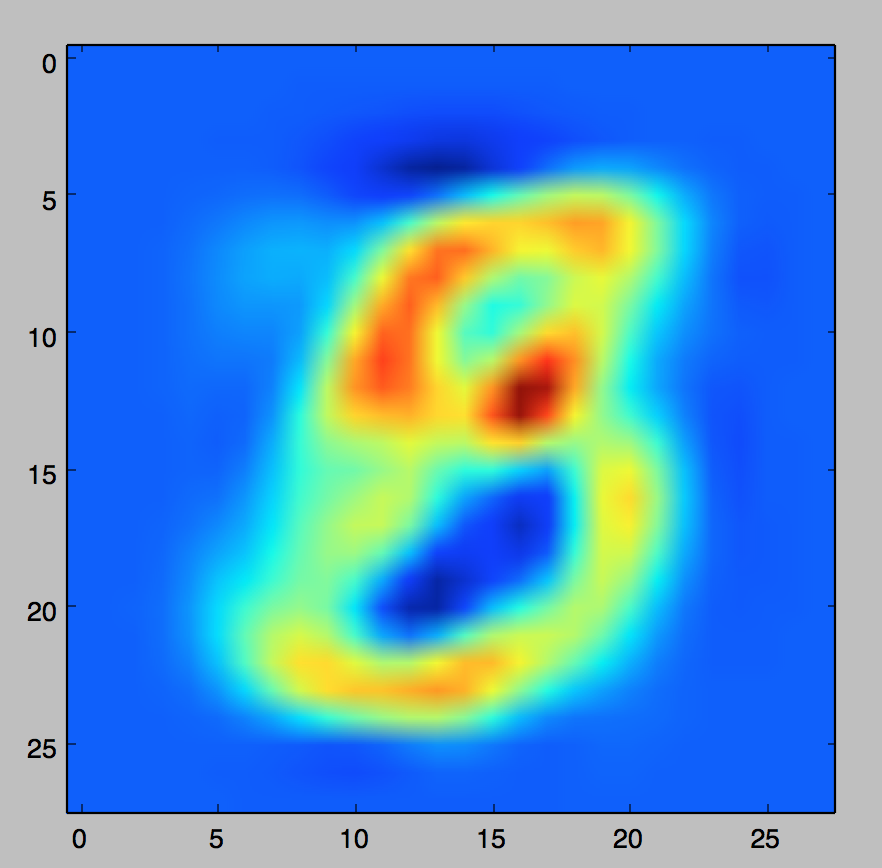
\includegraphics[scale=.15]{images/knn3_8_3.png} \\
\hline
9 & 4 & 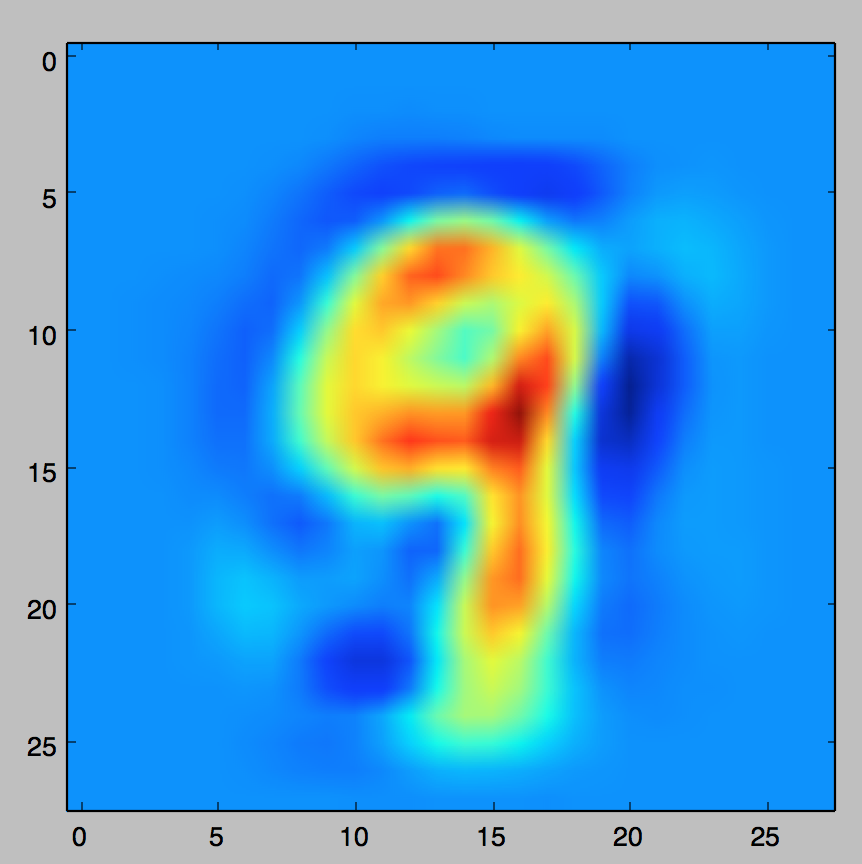
\includegraphics[scale=.15]{images/knn3_9_4.png} \\
\hline
\end{tabular}
\caption{Misclassified examples for K=3}
\label{ex:table}
\end{table}

\begin{table}[!th]
\centering
\begin{tabular}{|c|c|c|}
\hline
Class & Prediction & Image \\
\hline
0 & 5 & 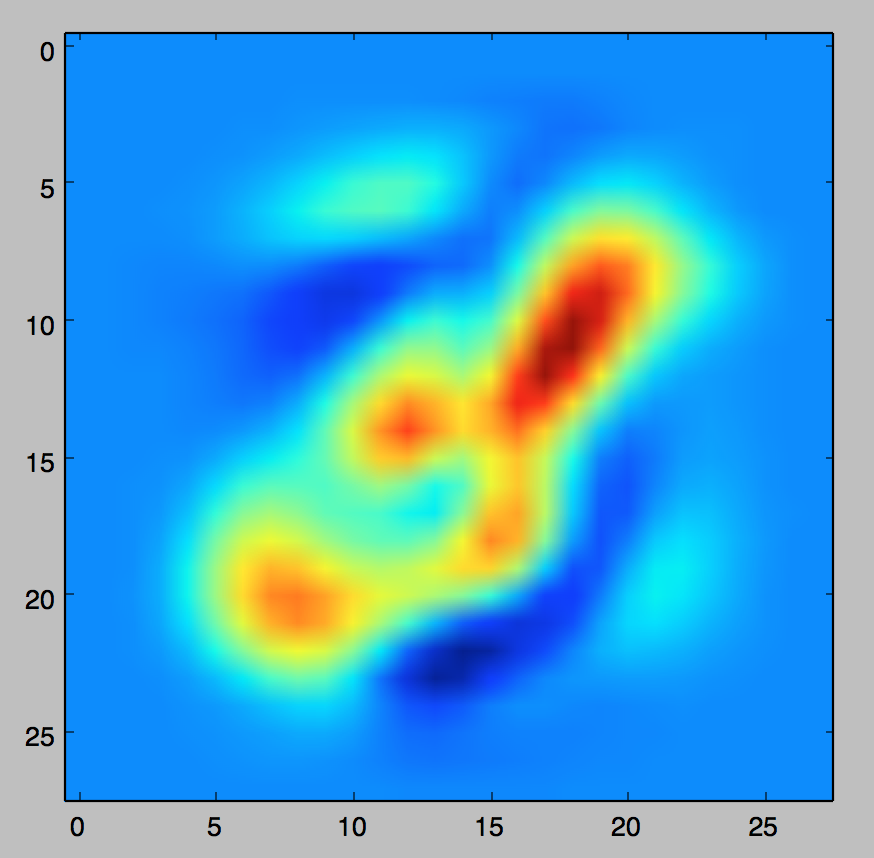
\includegraphics[scale=.15]{images/knn5_0_5.png} \\
\hline
5 & 6 & 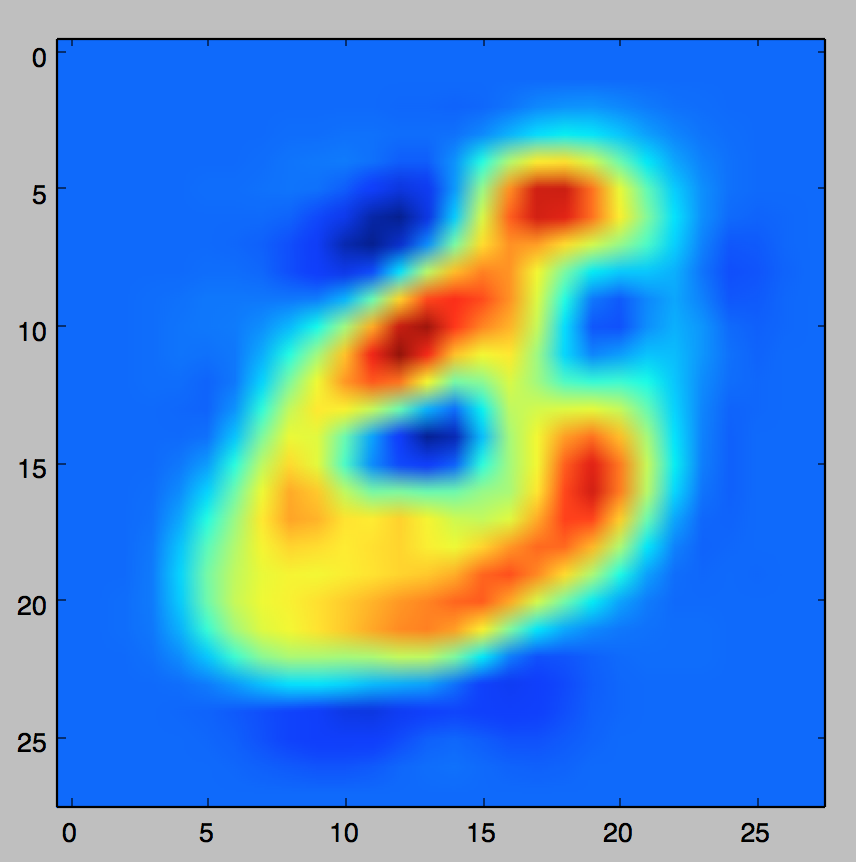
\includegraphics[scale=.15]{images/knn5_5_6.png} \\
\hline
7 & 2 & 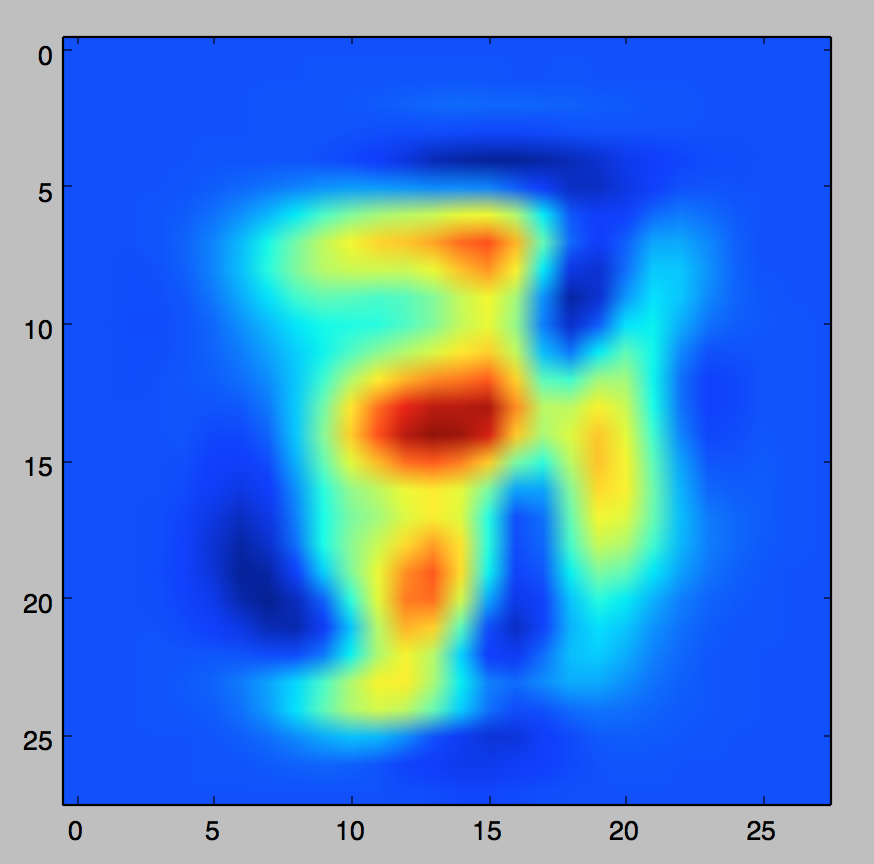
\includegraphics[scale=.15]{images/knn5_7_2.png} \\
\hline
\end{tabular}
\caption{Misclassified examples for K=5}
\label{ex:table}
\end{table}

\begin{table}[!th]
\centering
\begin{tabular}{|c|cccccccccc|}
\hline
 & 0 & 1 & 2 & 3 & 4 & 5 & 6 & 7 & 8 & 9 \\
\hline
0 & 48 & 0 & 0 & 1 & 0 & 1 & 0 & 0 & 0 & 0 \\
1 & 0 & 49 & 0 & 0 & 0 & 0 & 0 & 0 & 1 & 0 \\
2 & 0 & 0 & 48 & 0 & 1 & 0 & 1 & 0 & 0 & 0 \\
3 & 0 & 0 & 1 & 47 & 0 & 0 & 0 & 0 & 2 & 0 \\
4 & 0 & 0 & 0 & 0 & 48 & 0 & 0 & 0 & 1 & 1 \\ 
5 & 0 & 0 & 0 & 1 & 0 & 45 & 2 & 0 & 1 & 1 \\
6 & 0 & 0 & 0 & 0 & 1 & 5 & 43 & 0 & 0 & 1 \\ 
7 & 0 & 0 & 2 & 0 & 2 & 0 & 0 & 46 & 0 & 0 \\
8 & 0 & 0 & 1 & 0 & 0 & 1 & 0 & 0 & 47 & 1 \\
9 & 1 & 0 & 0 & 0 & 2 & 0 & 0 & 0 & 0 & 47 \\
\hline
\end{tabular}
\caption{Confusion Matrix for Bayes Classifier (Prediction accuracy = .936)}
\label{ex:table}
\end{table}

\begin{table}[!th]
\centering
\begin{tabular}{|c|c|}
\hline
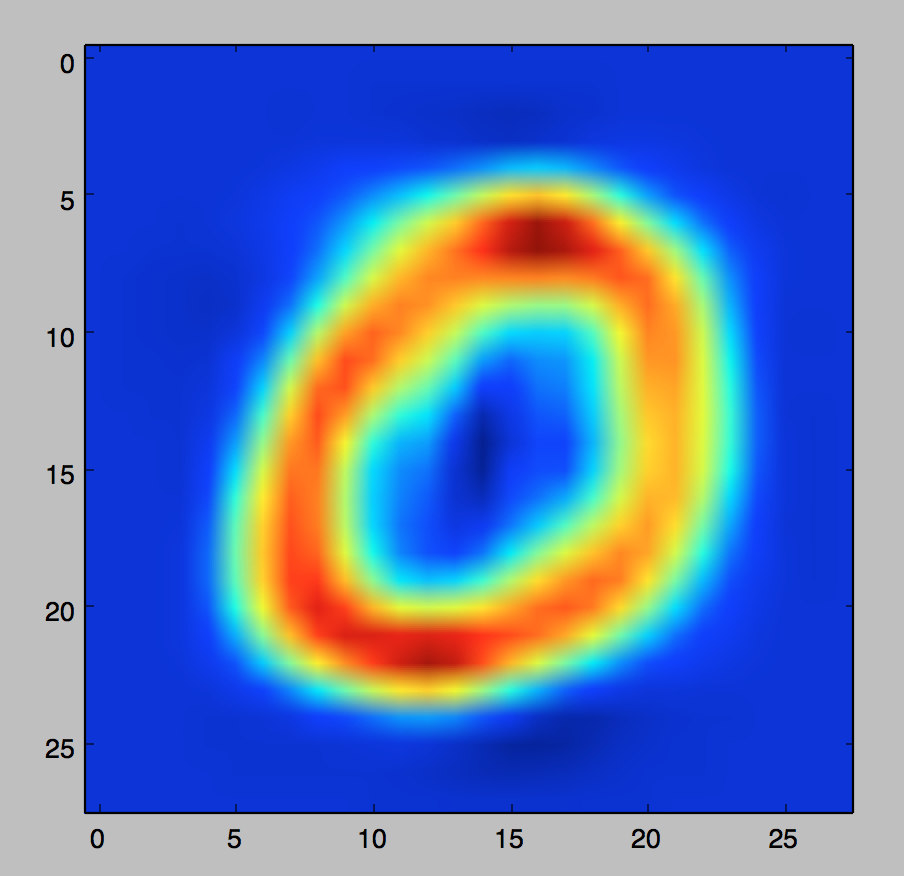
\includegraphics[scale=.15]{images/bayes0.png} & 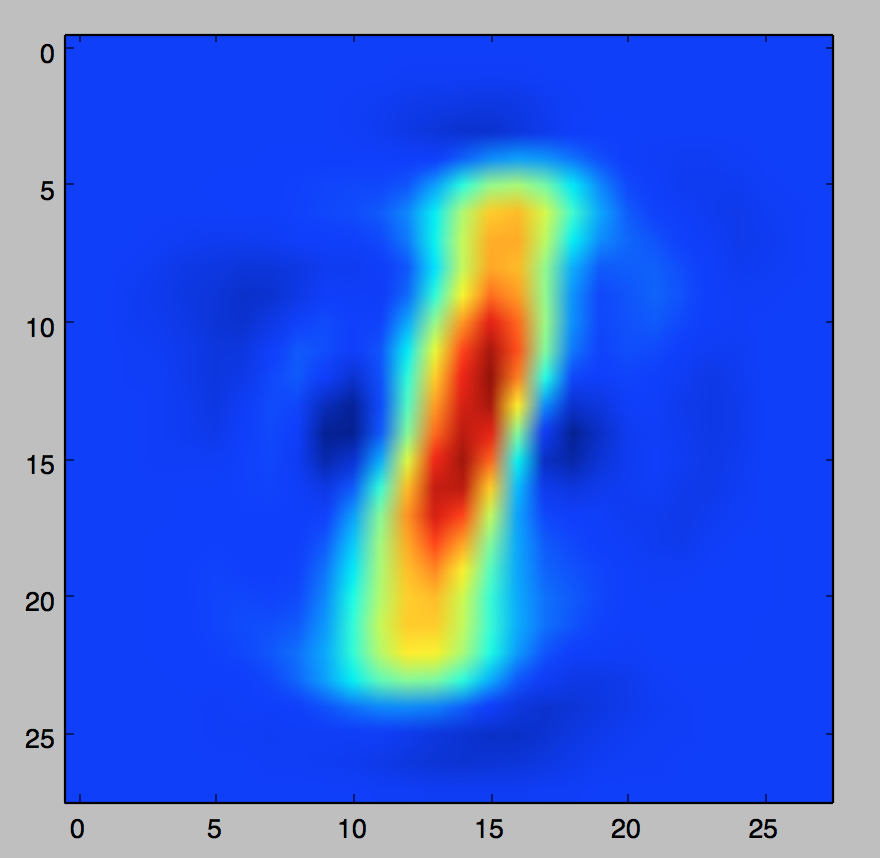
\includegraphics[scale=.15]{images/bayes1.png} \\
\hline
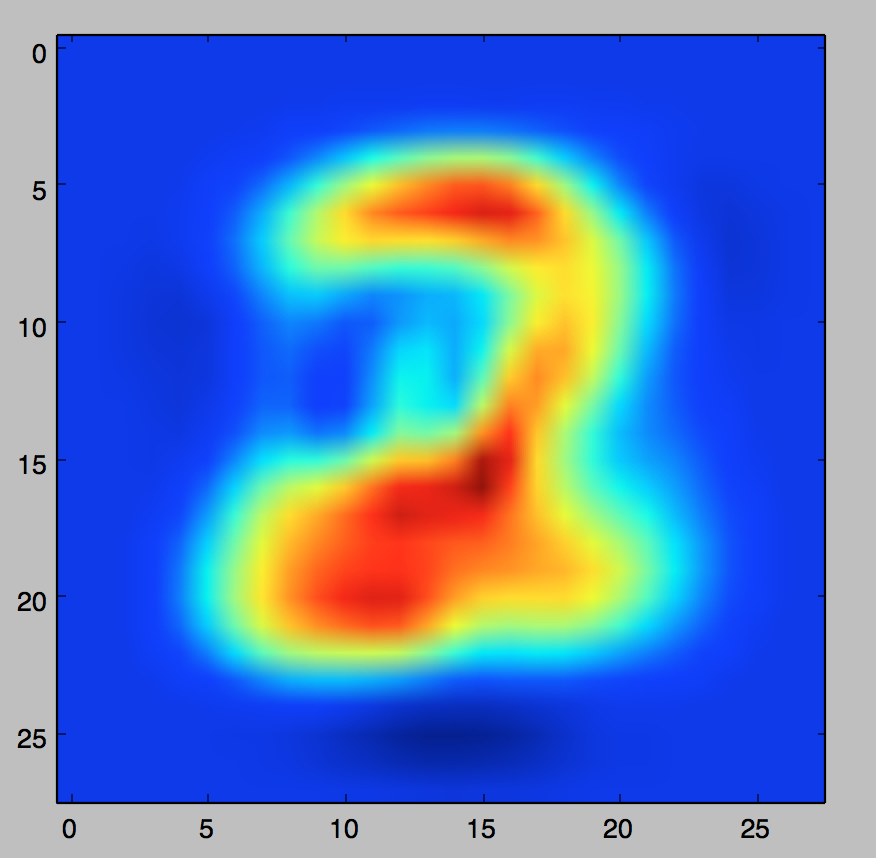
\includegraphics[scale=.15]{images/bayes2.png} & 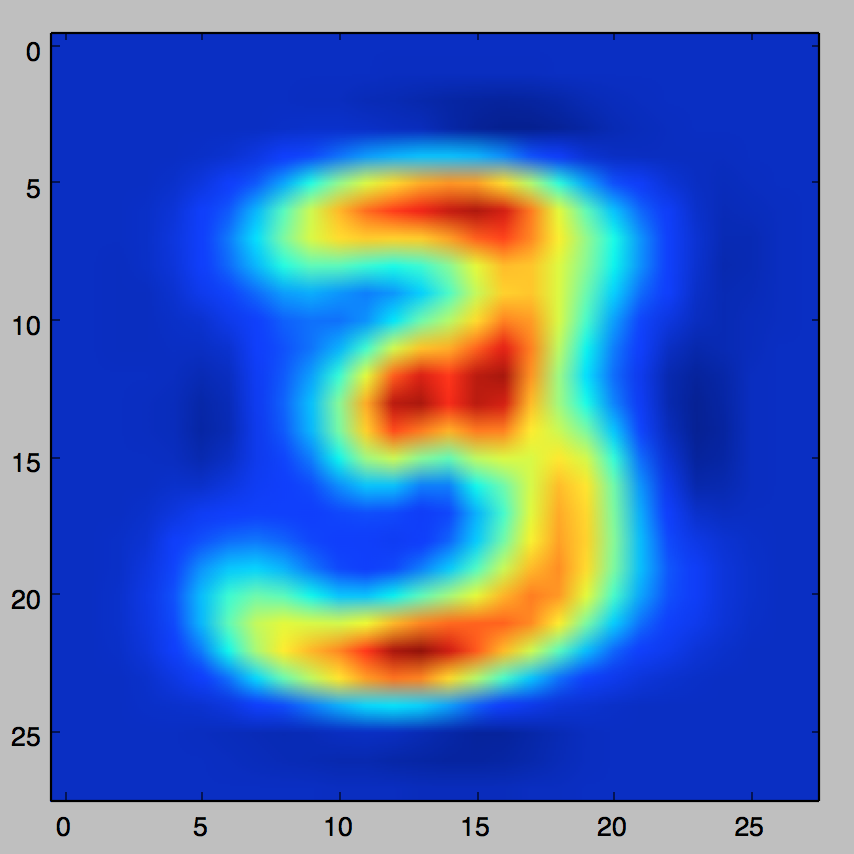
\includegraphics[scale=.15]{images/bayes3.png} \\
\hline
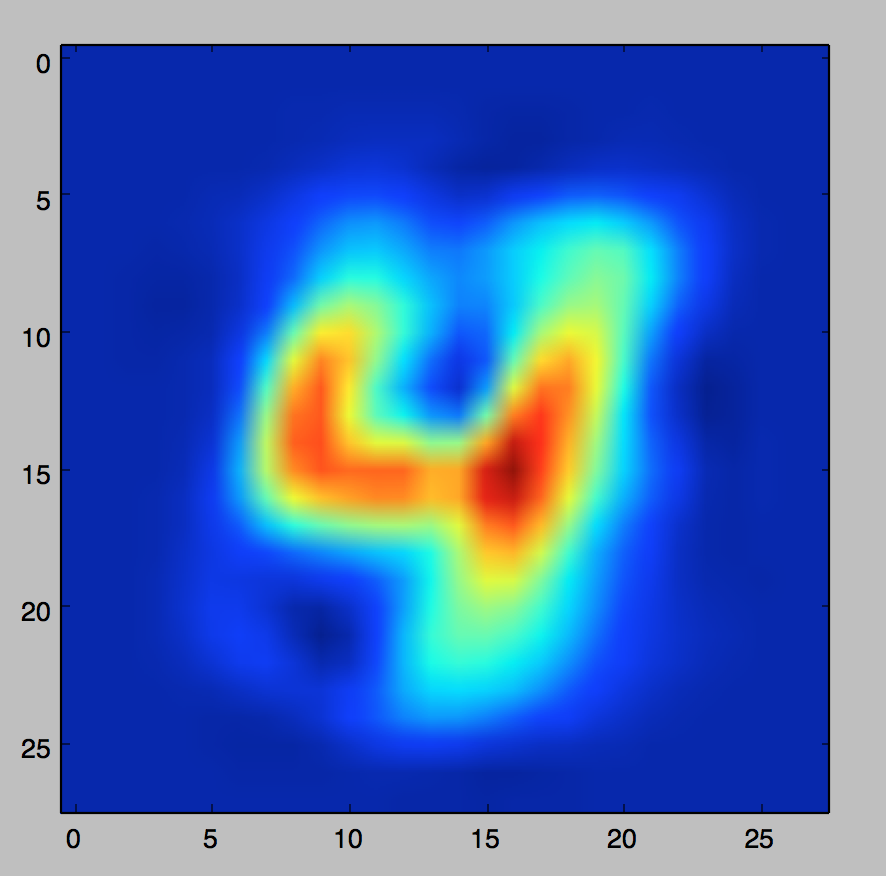
\includegraphics[scale=.15]{images/bayes4.png} & 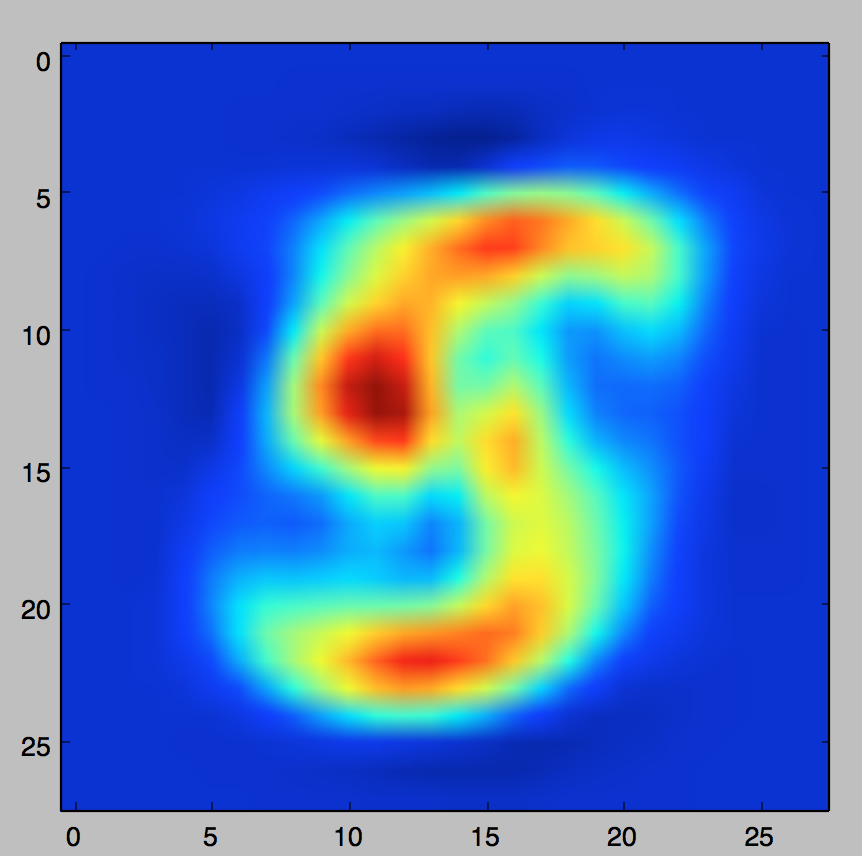
\includegraphics[scale=.15]{images/bayes5.png} \\
\hline
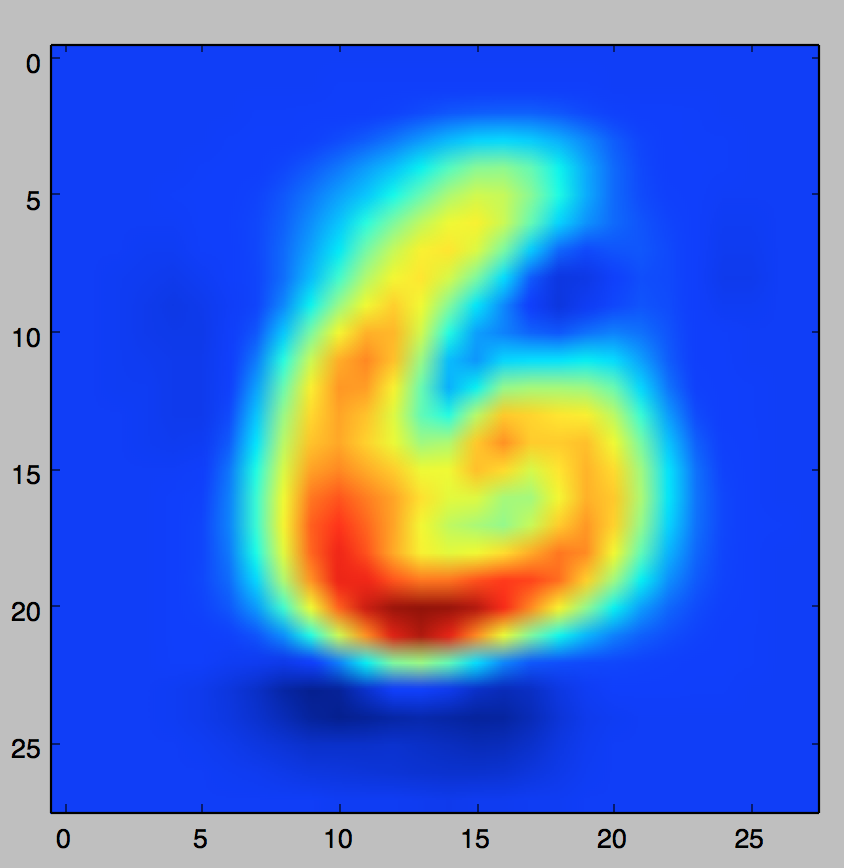
\includegraphics[scale=.15]{images/bayes6.png} & 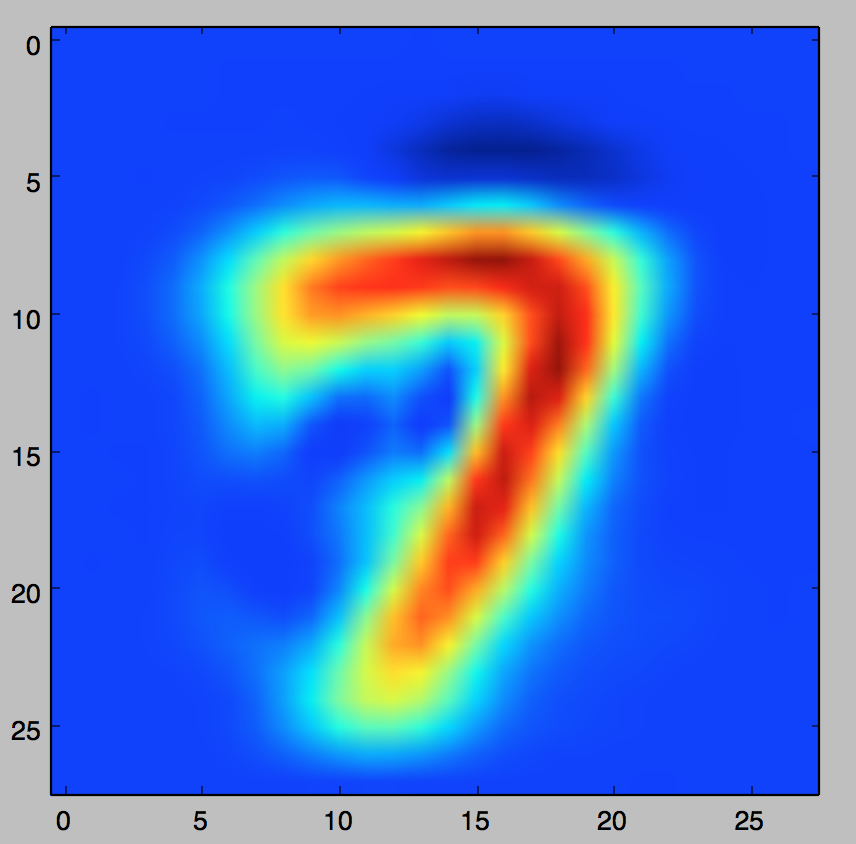
\includegraphics[scale=.15]{images/bayes7.png} \\
\hline
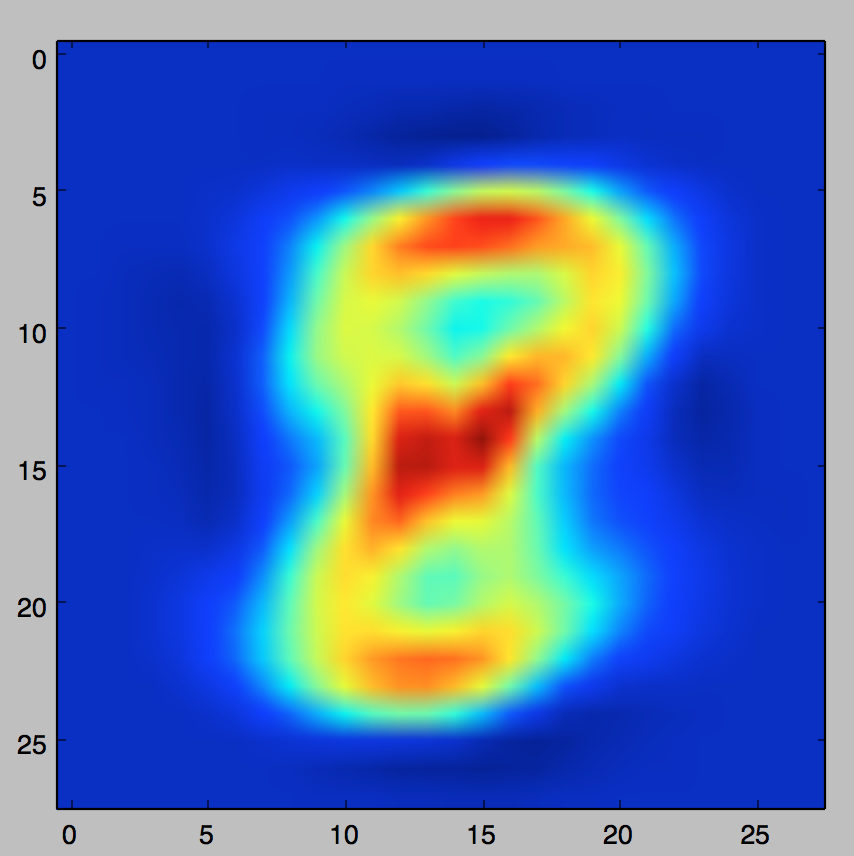
\includegraphics[scale=.15]{images/bayes8.png} & 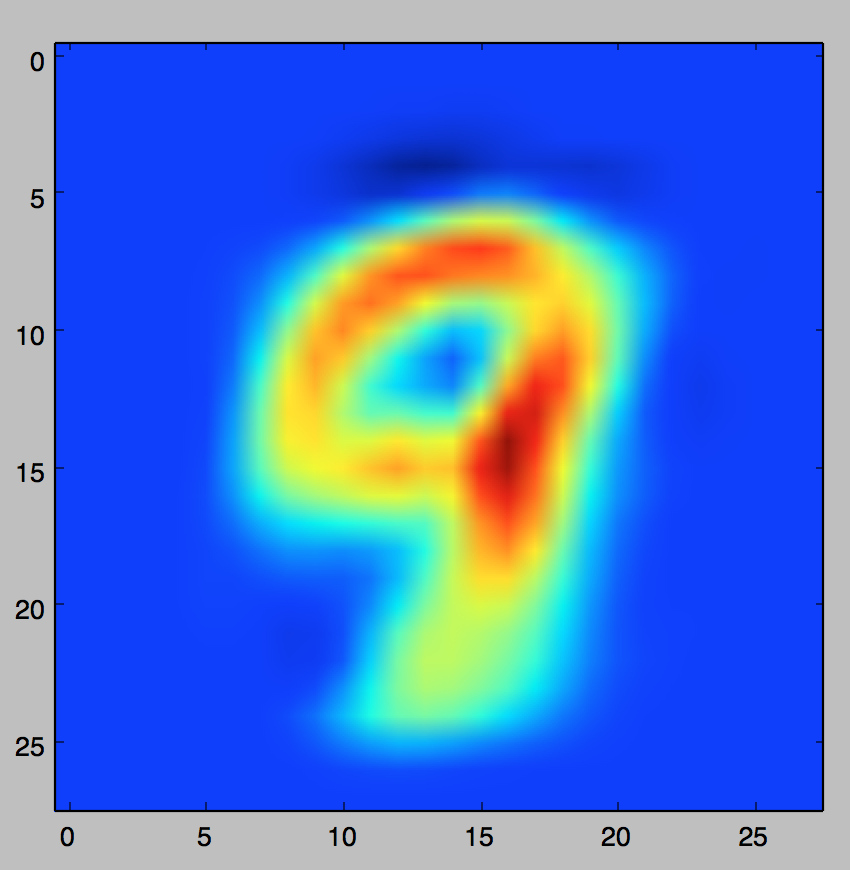
\includegraphics[scale=.15]{images/bayes9.png} \\
\hline
\end{tabular}
\caption{Image means for Bayes classifier}
\label{ex:table}
\end{table}

\begin{table}[!th]
\centering
\begin{tabular}{|clc|c||c|}
\hline
i & Class & Prediction & Image \\
\hline
84 & 1 & 8 & 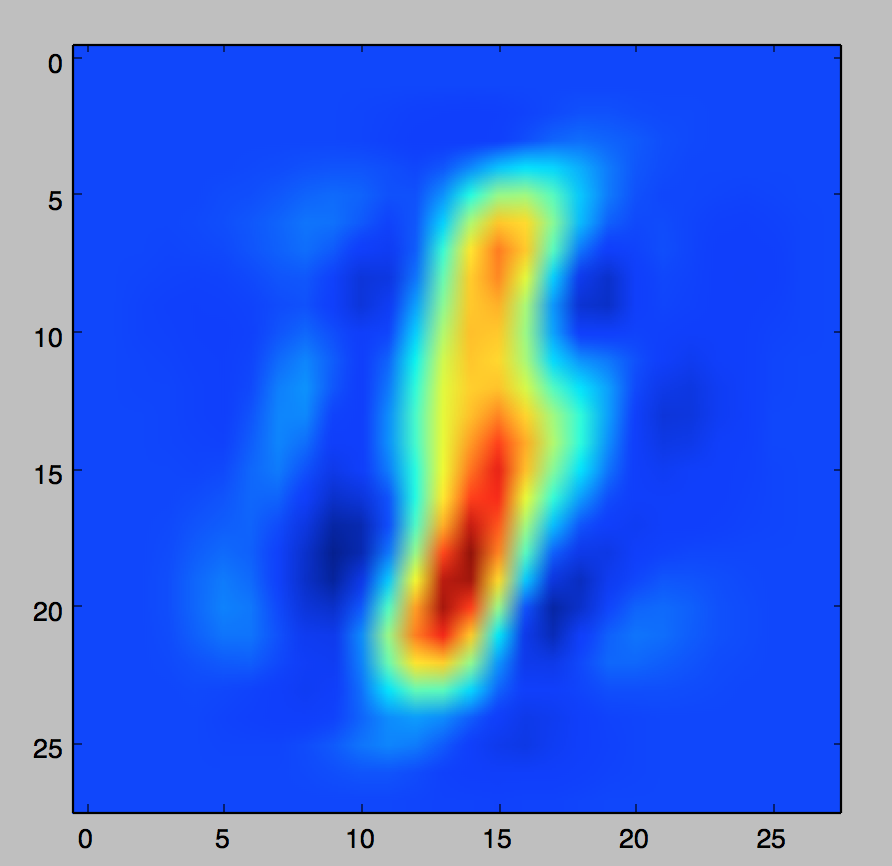
\includegraphics[scale=.2]{images/bayes_1_8.png} \\
\hline
189 & 3 & 2 & 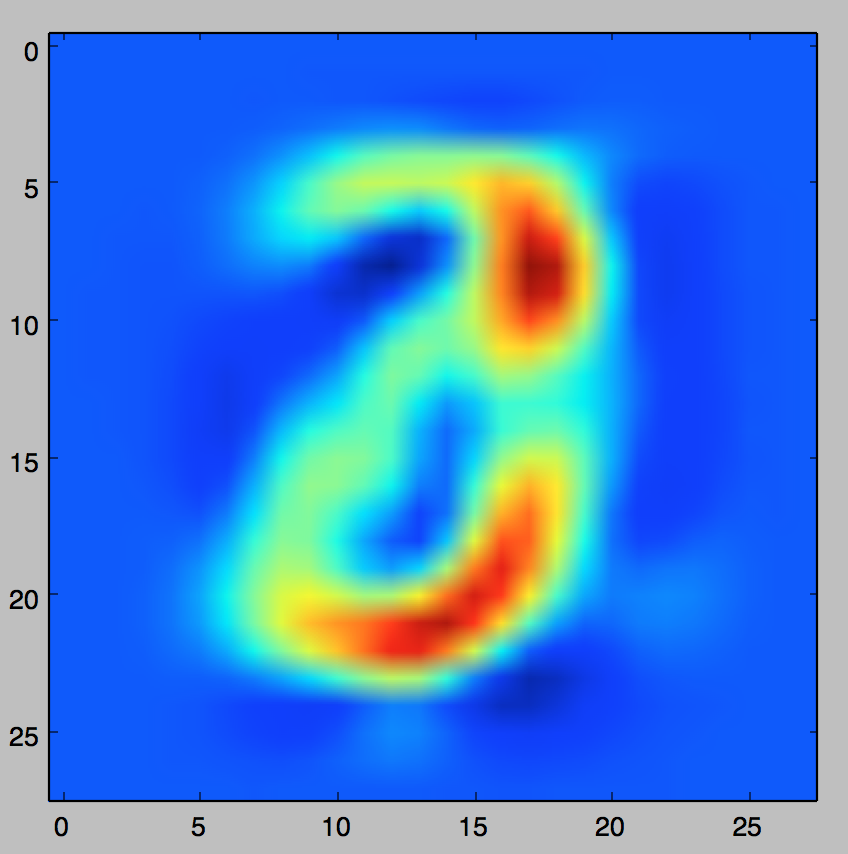
\includegraphics[scale=.2]{images/bayes_3_2.png} \\
\hline
456 & 9 & 0 & 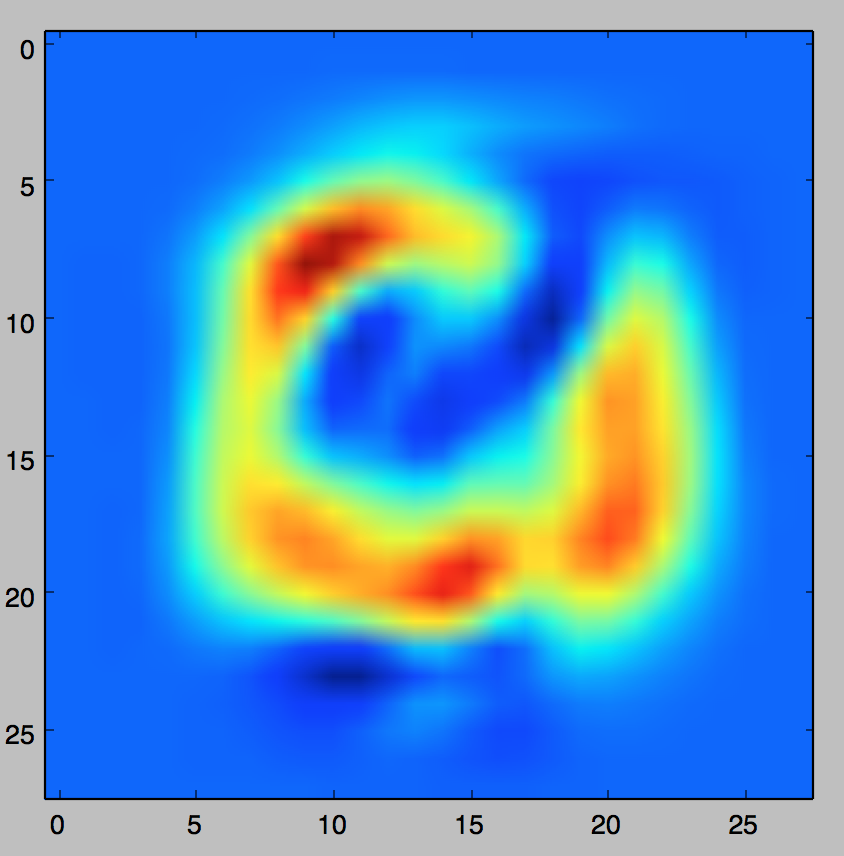
\includegraphics[scale=.2]{images/bayes_9_0.png} \\
\hline
\end{tabular}
\caption{Misclassified examples with Bayesian classifier}
\label{ex:table}
\end{table}

\begin{table}[!th]
\centering
\begin{tabular}{|c|c|}
\hline
Class & Likelihood \\
\hline
0 & 1.61427396527e-30 \\
1 & 0.000190440181997 \\
2 & 0.000184578956757 \\
3 & 1.57209260318e-08 \\
4 & 0.0013882095176 \\
5 & 2.43343185745e-13 \\
6 & 2.49257721585e-10 \\
7 & 5.52356463049e-09 \\
8 & 8.23010497024 \\
9 & 4.24372709689e-12 \\
\hline
\end{tabular}
\caption{Probability distributions for i=84}
\label{ex:table}
\end{table}

\begin{table}[!th]
\centering
\begin{tabular}{|c|c|}
\hline
Class & Likelihood \\
\hline
0 & 7.85200802045e-05 \\
1 & 5.53960717342e-132 \\
2 & 0.26868012579 \\
3 & 0.207323802348 \\
4 & 1.37871629701e-37 \\
5 & 7.0913139412e-13 \\
6 & 2.10121631612e-18 \\
7 & 8.64158255829e-51 \\
8 & 9.39609382955e-07 \\
9 & 3.50286382359e-24 \\
\hline
\end{tabular}
\caption{Probability distributions for i=189}
\label{ex:table}
\end{table}

\begin{table}[!th]
\centering
\begin{tabular}{|c|c|}
\hline
Class & Likelihood \\
\hline
0 & 1.01943498002e-09 \\
1 & 0.0 \\
2 & 4.77168981732e-13 \\
3 & 1.84914477161e-37 \\
4 & 2.09951907729e-33 \\
5 & 2.61861276808e-50 \\
6 & 3.49193403358e-23 \\
7 & 2.28328889615e-105 \\
8 & 3.81858520041e-39 \\
9 & 5.89572887373e-43 \\
\hline
\end{tabular}
\caption{Probability distributions for i=456}
\label{ex:table}
\end{table}

\begin{figure}[h]
\centerline{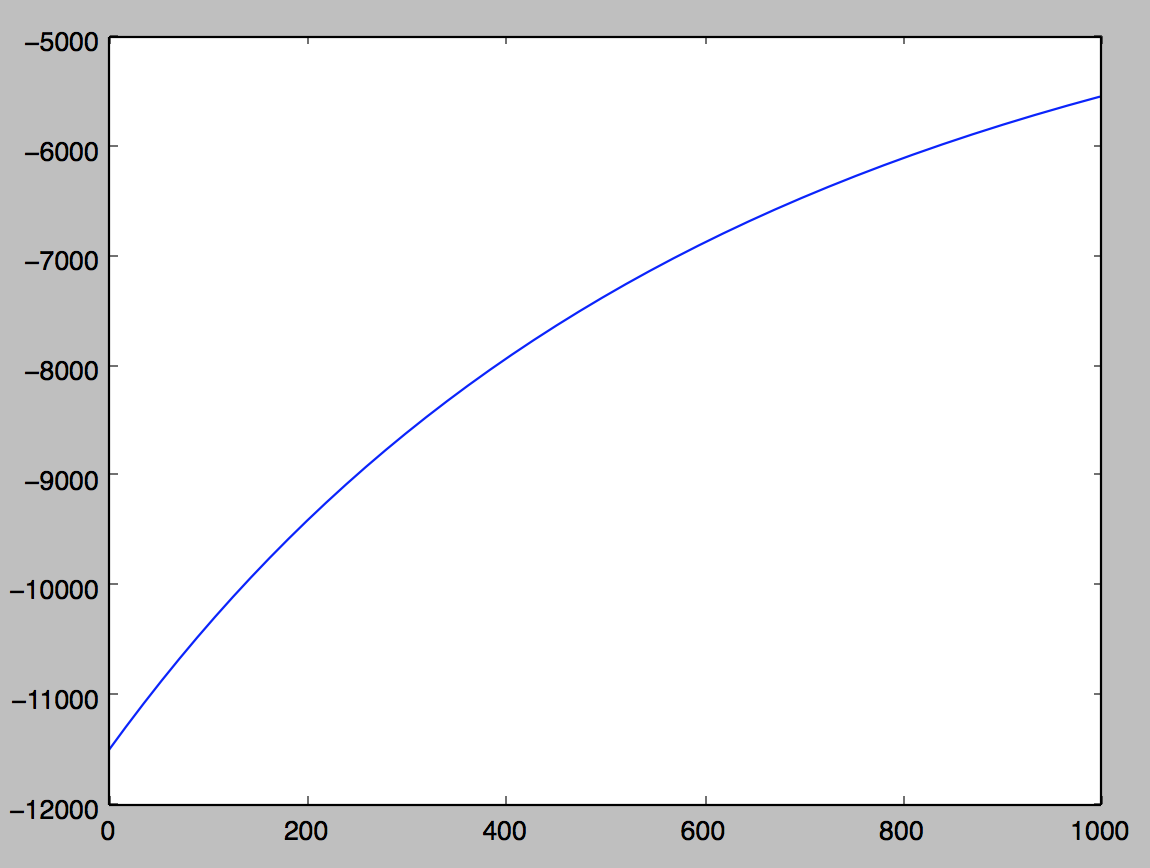
\includegraphics[scale=.6]{images/loglikelihood.png}}

\centerline{Plot of log likelihood error by number of iterations for Logistic Regression classifier.}
\end{figure}

\begin{table}[!th]
\centering
\begin{tabular}{|c|cccccccccc|}
\hline
 & 0 & 1 & 2 & 3 & 4 & 5 & 6 & 7 & 8 & 9 \\
\hline
0 & 42 & 0 & 1 & 1 & 0 & 2 & 3 & 0 & 1 & 0 \\
1 & 0 & 35 & 0 & 0 & 0 & 0 & 0 & 0 & 15 & 0 \\
2 & 1 & 0 & 36 & 3 & 0 & 0 & 3 & 0 & 7 & 0 \\
3 & 1 & 0 & 1 & 37 & 0 & 1 & 0 & 0 & 10 & 0 \\
4 & 0 & 0 & 1 & 0 & 33 & 1 & 0 & 0 & 5 & 10 \\
5 & 0 & 0 & 0 & 11 & 2 & 25 & 1 & 0 & 8 & 3 \\
6 & 0 & 0 & 1 & 0 & 6 & 2 & 37 & 0 & 4 & 0 \\
7 & 0 & 0 & 1 & 0 & 1 & 0 & 0 & 34 & 7 & 7 \\
8 & 0 & 0 & 0 & 0 & 0 & 2 & 0 & 0 & 47 & 1 \\
9 & 0 & 0 & 0 & 0 & 2 & 0 & 1 & 0 & 2 & 45 \\
\hline
\end{tabular}
\caption{Confusion Matrix for Logistic Regression (Prediction accuracy = 0.7419)}
\label{ex:table}
\end{table}

\begin{table}[!th]
\centering
\begin{tabular}{|clc|c||c|}
\hline
i & Class & Prediction & Image \\
\hline
275 & 5 & 3 & 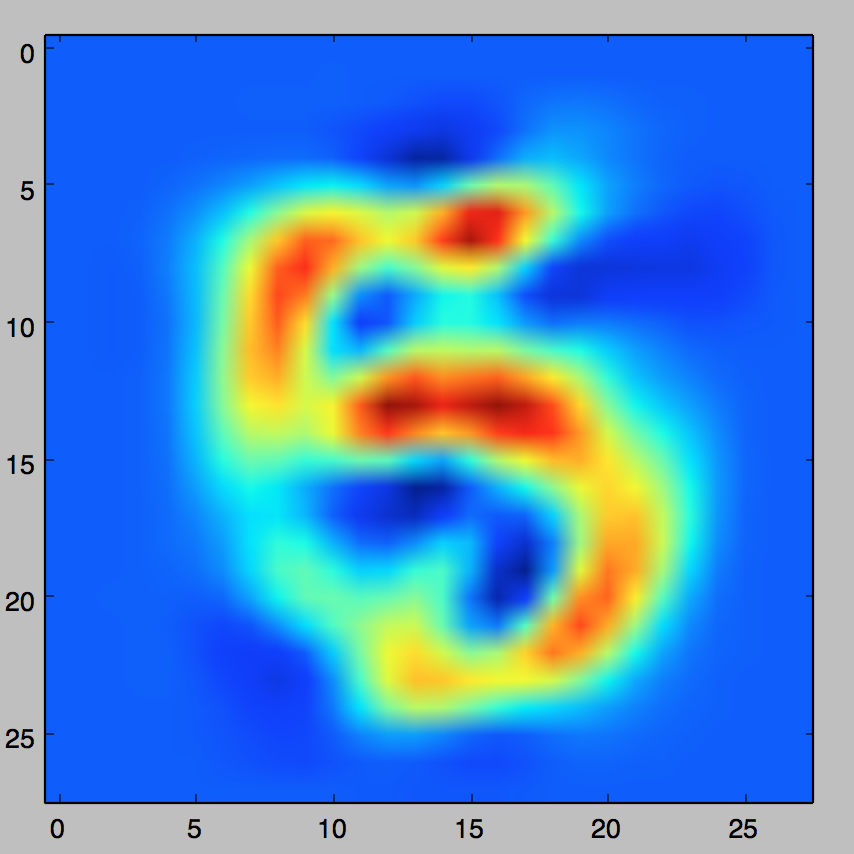
\includegraphics[scale=.2]{images/logit_5_3.png} \\
\hline
373 & 7 & 9 & 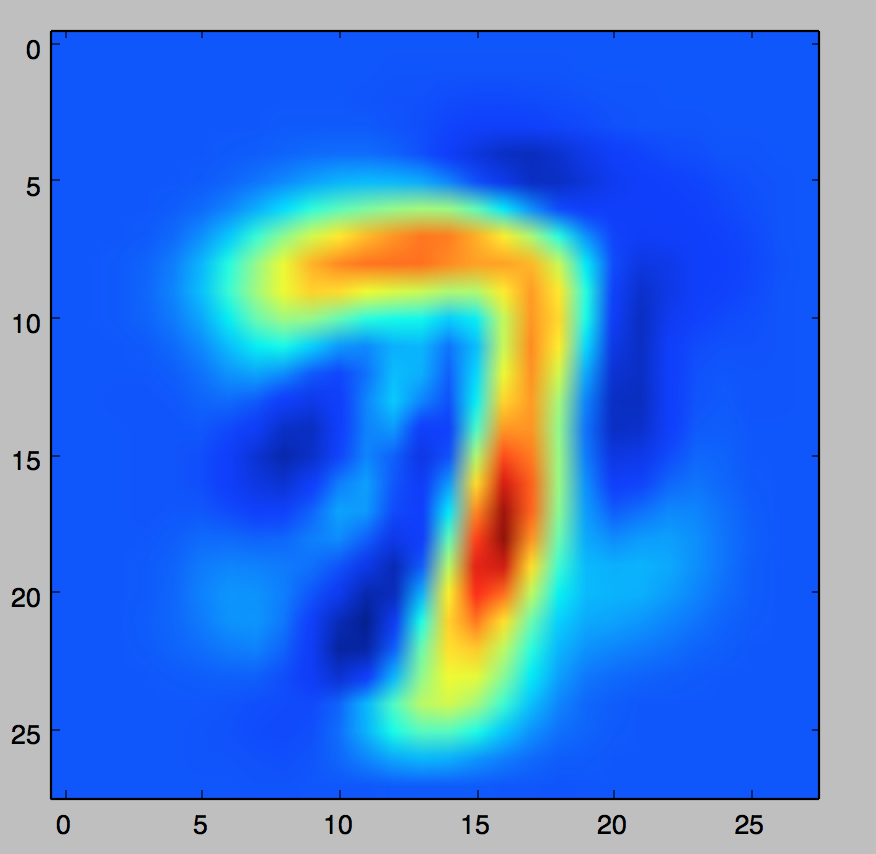
\includegraphics[scale=.2]{images/logit_7_9.png} \\
\hline
477 & 9 & 8 & 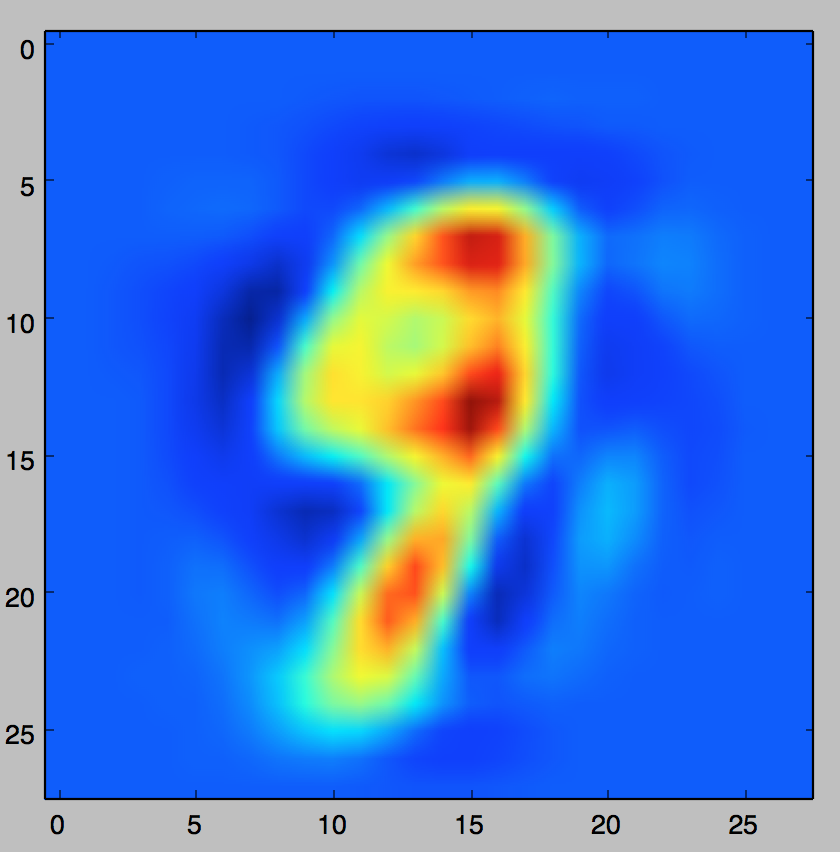
\includegraphics[scale=.2]{images/logit_9_8.png} \\
\hline
\end{tabular}
\caption{Misclassified examples with Logistic Regression classifier}
\label{ex:table}
\end{table}

\begin{table}[!th]
\centering
\begin{tabular}{|c|c|}
\hline
Class & Likelihood \\
\hline
0 & 0.056978 \\
1 & 0.005312 \\
2 & 0.054814 \\
3 & 0.279018 \\
4 & 0.054411 \\
5 & 0.170424 \\
6 & 0.064826 \\
7 & 0.024758 \\
8 & 0.178350 \\
9 & 0.111109 \\
\hline
\end{tabular}
\caption{Softmax probability distributions for i=275}
\label{ex:table}
\end{table}

\begin{table}[!th]
\centering
\begin{tabular}{|c|c|}
\hline
Class & Likelihood \\
\hline
0 & 0.011427 \\
1 & 0.004381 \\
2 & 0.043161 \\
3 & 0.096474 \\
4 & 0.061084 \\
5 & 0.061646 \\
6 & 0.017383 \\
7 & 0.309109 \\
8 & 0.081986 \\
9 & 0.313349 \\
\hline
\end{tabular}
\caption{Softmax probability distributions for i=373}
\label{ex:table}
\end{table}

\begin{table}[!th]
\centering
\begin{tabular}{|c|c|}
\hline
Class & Likelihood \\
\hline
0 & 0.009955 \\
1 & 0.128215 \\
2 & 0.039013 \\
3 & 0.112215 \\
4 & 0.039321 \\
5 & 0.150457 \\
6 & 0.037912 \\
7 & 0.068410 \\
8 & 0.256989 \\
9 & 0.157514 \\
\hline
\end{tabular}
\caption{Softmax probability distributions for i=477}
\label{ex:table}
\end{table}


\end{document}
